%!TEX root = SISC_elastic_3d.tex
\subsection{LOH.1 model problem with layered material}
As the final numerical example, we consider the layer-over-halfspace benchmark problem LOH.1 \cite{Day2001}. The computational domain is taken to be $(x,y,z)\in[0,30000]^2\times[0,17000]$ with a free surface boundary conditions at $z=0$.   The problem is driven by a single point moment source defined as 
$g(t,t_0,\omega) \mathcal{M} \cdot \nabla\delta (\mathbf{x}-\mathbf{x_0})$, 
where the point source location is $\mathbf{x_0}= (15000, 15000, 2000)$  and the moment time function is
\[g(t,t_0,\omega) = \frac{\omega}{\sqrt{2\pi}}e^{-\omega^2(t - t_0)^2/2}, \ \ \ \omega = 16.6667,\ \ \ \ t_0 = 0.36.\]
In the 3-by-3 symmetric moment tensor $\mathcal{M}$, the only nonzero elements are $\mathcal{M}_{12}=\mathcal{M}_{21}=10^{18}$.

The LOH.1 model has a layered material property with a material discontinuity at $z=1000$, with the dynamic and mechanical parameters given in Table \ref{material_parameter}. In the top layer $z\in [0, 1000]$, both the compressional and shear velocity are lower than the rest of the domain. For computational efficiency, a smaller grid spacing shall be used in the top layer. 

\begin{table}[htbp]
	\begin{center}
		\begin{tabular}{c c c c c}
			\hline
			~   & Depth $[m]$& $V_p[m/s]$ & $V_s [m/s]$ & $\rho[Kg/m^3]$ \\
			\hline
			Layer&0--1000& 4000& 2000& 2600\\
			half-space &1000--17000 & 6000 & 3464& 2700\\
			\hline 
		\end{tabular}
	\end{center}
	\caption{Dynamic and mechanical parameters for the layer and the lower half-space of the layer over half-space test.}\label{material_parameter}
\end{table} 

We solve the LOH.1 model problem by using the open source code SW4, where our proposed method has been implemented. The solution is recorded in a receiver on the free surface at the point $(x, y, z) = (21000, 23000, 0)$. The time history of the vertical, transverse and radial velocities are shown in Figure \ref{loh1_100} with grid spacing $h = 100$ in the half-space and $h/2 = 50$ in the top layer. Even though the smallest number of grid points per wavelength is only 5.22, the numerical solutions agree well with the exact solution. In Figure \ref{loh1_50}, the solutions computed on a finer mesh with $h = 50$ in the half-space and $h/2 = 25$ in the top layer look identical to the exact solutions.
\begin{figure}[htbp]
	\centering
	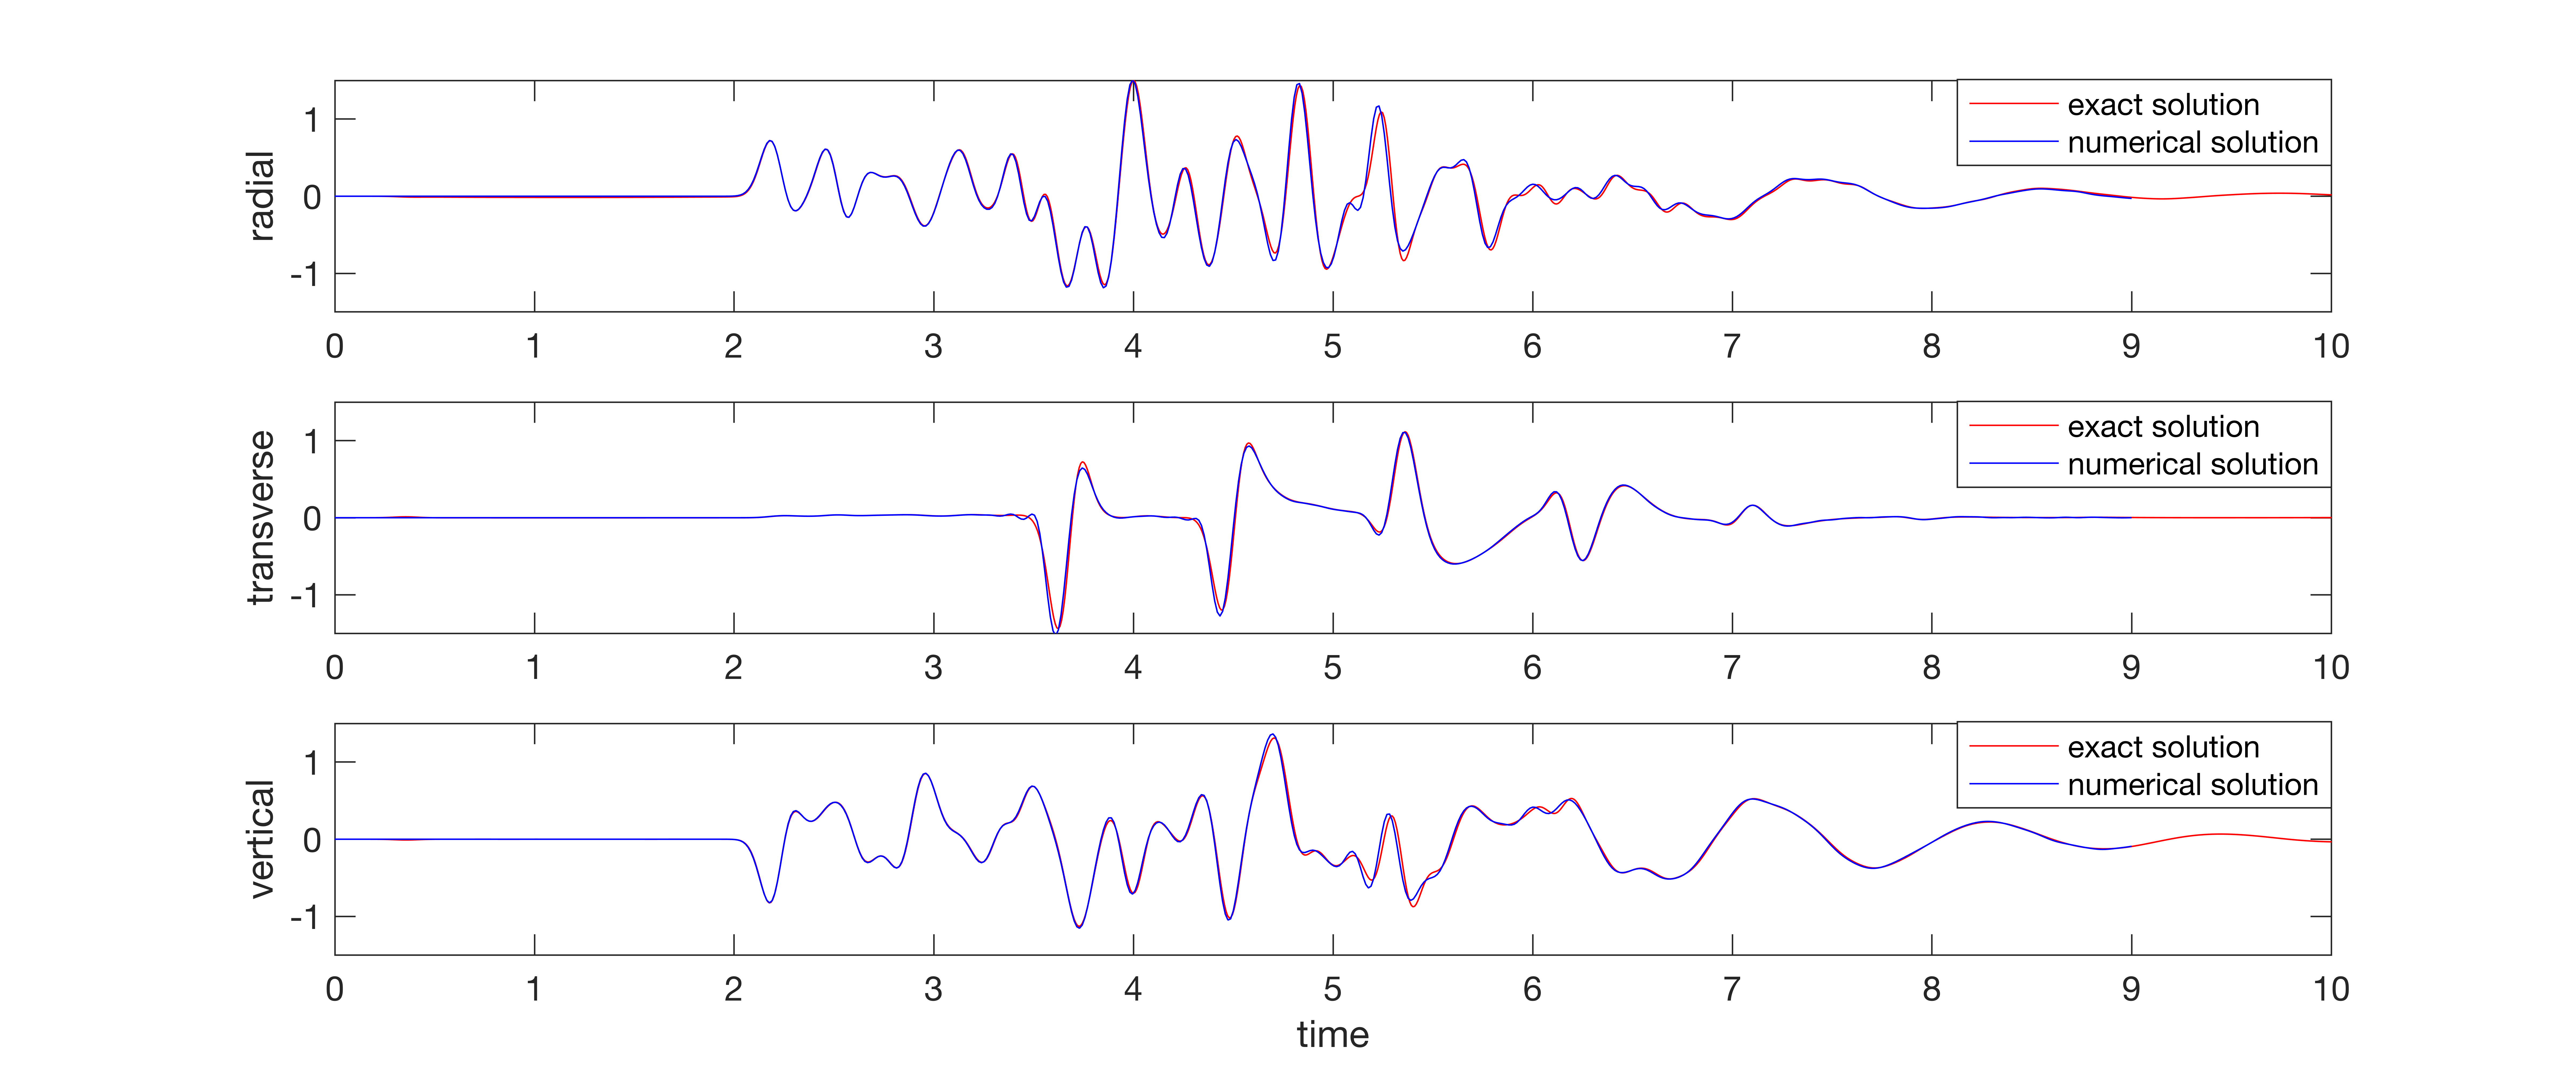
\includegraphics[width=0.9\textwidth,trim={4cm 0.2cm 4cm 1.5cm}, clip]{loh1_h100.png}
	\caption{LOH.1: The radial (top), transverse (middle), and vertical (bottom) velocities time histories. Here the numerical solutions are plotted in blue ($h = 100$) and the semi-analytical solution is plotted in red.}\label{loh1_100}
\end{figure}

\begin{figure}[htbp]
	\centering
	\includegraphics[width=0.9\textwidth,trim={4cm 0.2cm 4cm 1.5cm}, clip]{loh1_h50.png}
	\caption{LOH.1: The radial (top), transverse (middle), and vertical (bottom) velocities time histories. Here the numerical solutions are plotted in blue ($h = 50$) and the semi-analytical solution is plotted in red.}\label{loh1_50}
\end{figure}

To test the performance of the new method, we record the quotient between the computational time of solving the linear system for the mesh refinement interface and of the time-stepping procedure in Table \ref{time}. We have run simulations on two different computer clusters. First, we use two nodes on the Rackham cluster with each node consisting of two 10-core Intel Xeon V4 CPUs and 128 GB memory. In the second simulation, we use three nodes on ManeFrame II (M2) with each node consisting of two 18-core Intel Xeon E5-2695 v4 CPUs and 256 GB memory. From Table \ref{time}, we observe that our new method (with ghost points from the coarse domain) needs much less time to solve the linear system for interface conditions compared with the old method in SW4 (with ghost points from both coarse and fine domains). 

\begin{table}[htbp]
	\begin{center}
		\begin{tabular}{|c|c|c|}
			\hline
			Machine   & new method & old method \\
			\hline
			Rackham & 4.02\% &  8.16\%\\
			\hline
			M2 &5.17\% & 8.87\%\\
			\hline 
		\end{tabular}
	\end{center}
		\caption{The quotient of the computational time of solving the linear system for the mesh refinement interface and of the time-stepping procedure}\label{time}
\end{table} 

In addition, the proposed method implemented in SW4 has excellent parallel scalability. When running the same model problem with 4 nodes (80 cores) on the Rackham cluster, the computational time of the time stepping procedure is $51\%$ of that with 2 nodes. 
